\section{Bridges in HECRAS and \anuga{} (using internal boundary operators)}
This test compares a prismatic channel flow with a bridge in HECRAS and ANUGA.
A 10m wide, 1000m long channel (slope of 1/200, bankfull depth of 1m,
rectangular cross-section) flows through a floodplain (10m wide on either side
of the channel) (Figure~\ref{schematic}). 500m downstream there is a bridge
with a 1.3m high rectangular opening over the channel, and a deck elevation of
-1m. In HECRAS the bridge is modelled using the enegy method, see the
associated HECRAS files for details. In ANUGA the bridge is modelled by
inserting the bridge deck (upper chord) into the topography, with an internal
boundary operator to describe the bridge underflow. The rating curves were
derived from HECRAS by raising the upper chord of the bridge (far about the
flow) and computing internal boundary tables.  The bridge overflow in ANUGA is
modelled with the shallow water equations (although riverwalls could also be
used to apply weir type equations instead). Both models have a uniform
Manning's n of 0.045, which prevents too much supercritical flow in HECRAS (and
the associated numerical supression of the inertial terms that HECRAS uses to
retain stability).

\begin{figure}
\begin{center}
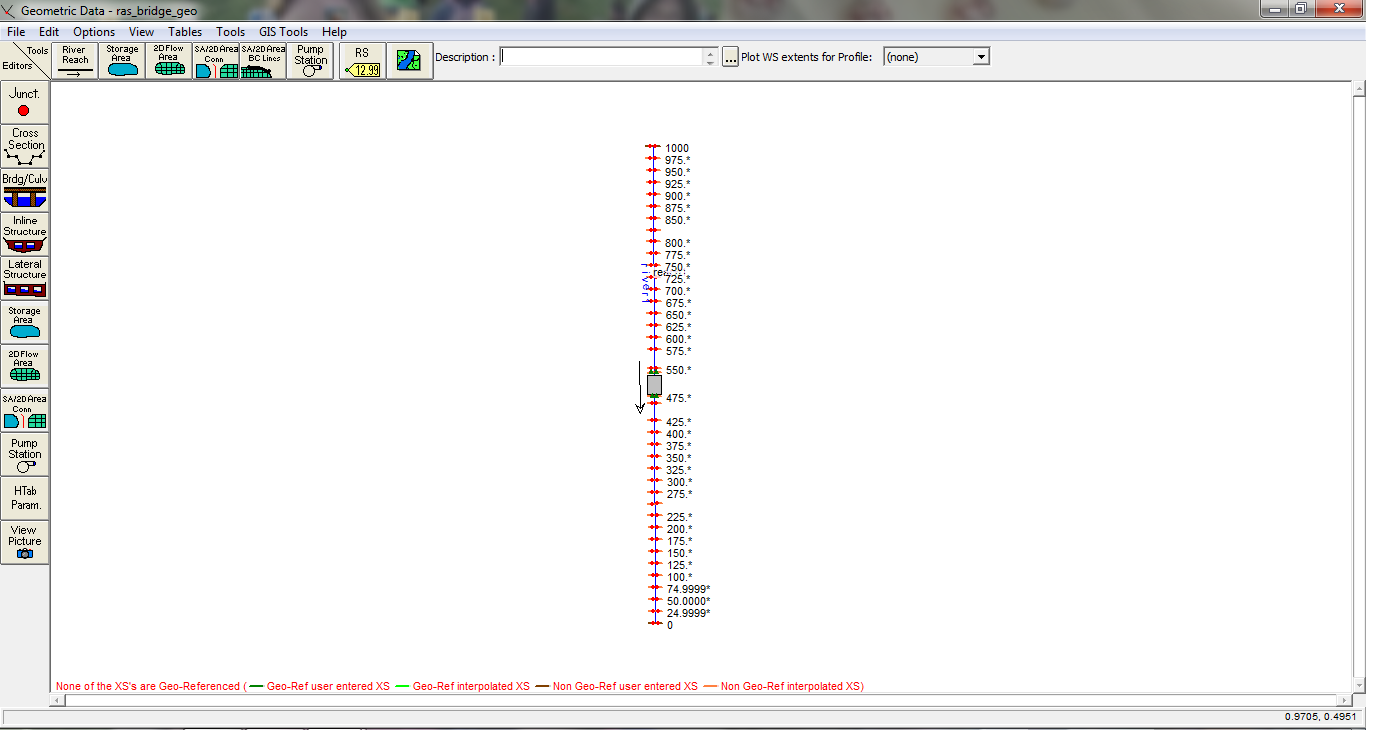
\includegraphics[width=1.0\textwidth]{hecras_bridge_test/RASGeometry_Bridge.png}
\end{center}
\caption{Screenshot showing the HECRAS model geometry schematization}
\label{schematic}
\end{figure}


A discharge timeseries is imposed upstream for both models, with the discharge
increasing from 1m$^3$/s initially to 70m$^3$/s at the end of the simulation.
Details of the model setup can be seen in the code / input files in this
directory.

\subsection{Results}

Figure~\ref{Reach} show stage timeseries at various stations downstream in each
model. The ANUGA and HECRAS results are qualitatively similar, but differ in
detail. In early stages of the simulation when discharges are lower, ANUGA
shows stages slightly below HECRAS. This reflects the fact that HECRAS models
side-wall friction while ANUGA does not, so there is more drag in the HECRAS
model. As the discharge increases, the models show more deviation around the
bridge and upstream, and ultimately approach different steady states. The main
reason for this is that they use different methods to model the bridge
overflow, which begins when station 525 exceeds -1m. Another cause of
differences is that in HECRAS, stage over all cross-sections is constant,
including just upstream and downstream of the bridge. On the other hand in
these locations ANUGA predicts some cross-channel variations in channel and
floodplain stage. This is caused by the flux of water under the centre of the
bridge. Just upstream of the bridge, ANUGA predicts the stage in the channel is
slightly lower than on the floodplains, whereas the reverse is true just
downstream, as would be expected from the bridge underflow. Combined with the
fact that ANUGA's enquiry points for the bridge underflow rating curves occur
in the centre of the channel, we cannot expect exact agreement with HECRAS.
HECRAS includes several other bridge models, and these would also give
different results particularly when the bridge deck is inundated. 

\begin{figure}
\begin{center}
\includegraphics[width=0.9\textwidth]{CENTRAL_CHANNEL.png}
\end{center}
\caption{Stage at various points downstream in the channel}
\label{Reach}
\end{figure}

